\documentclass[a4paper,10pt]{article}
\usepackage[portugues]{algorithm2e}
%linguagem
\usepackage[brazil]{babel}
%encodificação
\usepackage[utf8]{inputenc}
\usepackage{float}
%biblioteca de matemática
\usepackage{amssymb,amsmath}
%pacote para codigo fonte
\usepackage{listings}
%mostra o nome em cima
\pagestyle{headings}
%figuras
\usepackage{graphicx}
%cores
\usepackage{color}
%paragrafo no inicio da secao
\usepackage{indentfirst}
%usa pacote algoritmo
\usepackage{caption}
\usepackage{subcaption}
\usepackage{framed}
\usepackage[hmargin=2cm,vmargin=3.5cm,bmargin=2cm]{geometry}



%define a cor "claro"
\definecolor{claro}{gray}{0.9}

%configurações do listings
\lstset{frame=trBL, numbers=left, xleftmargin=-10pt, xrightmargin=-10pt,
breaklines=true,basicstyle=\footnotesize\ttfamily}
\begin{document}


\title{\textbf{Universidade Federal de Minas Gerais}\\
		Trabalho Prático: Oficina de Eletrodomésticos\\
		Engenharia de Software}

\author{Guilherme Nascimento\\
	Marcelle Yitse\\
	Lucas Augusto\\
	Willer\\
}
	
\date{\today}  %\today is replaced with the current date
\maketitle


\section{Introdução }
O trabalho a seguir consiste na implementação de um software de gerenciamento de uma oficina de eletrodomésticos. Para a realização desse trabalho foi necessário a aplicação dos diversos conceitos aprendidos na disciplina de Engenharia de Software tais como a elaboração dos requisitos, definição do modelo de processo, arquitetura e diagramas para a compreensão do projeto tanto para o cliente como para os desenvolvedores. Por fim, todo o programa é implementado na linguagem Java e por fim submetida a testes de validação para ser entrega na data final estipulada.

O sistema de gerenciamento aqui descrito suporta atividades CRUD: Cadastro, remoção e atualização para clientes, eletrodomésticos, peças, contatos de fabricantes e os próprios funcionários utilizadores do sistema.

Este documento está dividido em 7 seções das quais temos: contextualização, modelo de processo e cronograma, especificação de requisitos, projeto arquitetural, detalhes de projeto, comentarios da implementação e por fim, conclusão.


\section{Modelo de Processo}
\subsection{Modelo Cascata}

O modelo cascata foi escolhido pela equipe devido ao nível de complexidade do sistema a ser criado não ser grande e por todos os requisitos serem bem definidos. O sistema constitui numa aplicação desktop, logo o cascata favorece nesse sentido, pois caso haja falhas no processo de elicitação de requisitos, o que acarretará uma mudança no sistema já criado, implicará na criação de uma nova versão e com isso uma nova visita ao cliente para realizar a implantação do sistema. 

Como o cascata possui seus requisitos bem definidos na documentação e essa parte sendo a principal, ele garantirá a minimização de falhas durante o processo de desenvolvimento e seguirá de forma rigorosa a documentação para atender ao máximo o objetivo do cliente. 

Caso haja alguma mudança a ser feita, será realizada uma nova fase de documentação, estudo de viabilidade e  análise de requisitos para depois ser feita uma nova versão e logo em seguida a sua implantação no ambiente do cliente.

\subsection{Responsabilidades e Cronograma}

O cronograma abaixo aborda todo o processo necessário para o desenvolvimento do software de gerenciamento, o tempo total demandado foi de 7 semanas, onde todos elementos da equipe participaram do procedimento, composto por  etapas de análise de requisitos, projeto arquitetural, documentação, criação de diagramas UML e de cenários de uso, Implementação e testes unitários, fase esta onde todos elementos da equipe participam, testes de integração, documentação final e manutenção, período este que perdura enquanto o software for utilizado.

\begin{figure}[H]
\centering
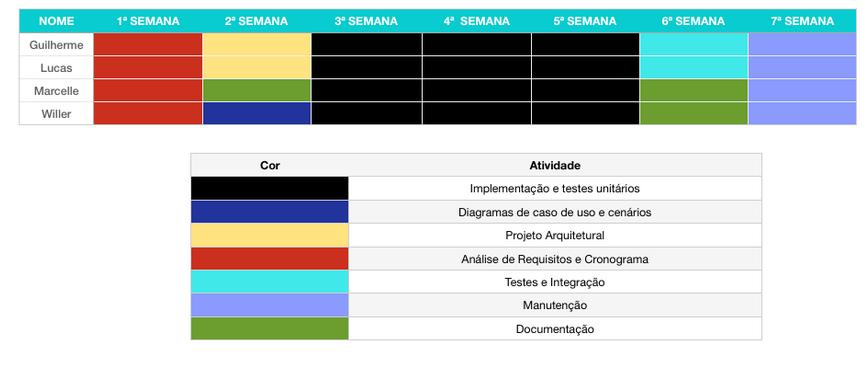
\includegraphics[width=1\textwidth]{pic/cronograma.jpeg}
\end{figure}

\section{Especificação de Requisitos}

Para fazer a especificação de requisitos foi imaginado um cenário de comunicação entre o cliente e o grupo a fim de dar detalhes do sistema que gerenciará a oficina de eletrodomésticos.	

\subsection{Contextualização}

Com o atual auxílio da informática, automatizar sistemas e processos arcaicos significa otimizar gastos, tempo e manter uma organização sobre o seu trabalho. Uma oficina de eletrodomésticos possui muito a ganhar ao automatizar seu sistema de gerenciamento, status de produtos na oficina, controle de notas fiscais, controle das finanças da empresa e também dos funcionários facilita a vida do gerente. 

A presença de um sistema que possa agregar todas essas funcionalidades citadas acima poderá aumentar a qualidade dos serviços ofertados pela oficina, otimizar o tempo gasto com tarefas burocráticas, manter organizado todo ecossistema da mesma e garantir que o empresário dono da oficina atinja e atenda mais clientes, de uma maneira otimizada e segura. 

\subsection{Análise de viabilidade}

Com as condição estipuladas, os desenvolvedores e projetistas definiu o projeto como viável, sendo necessário não mais que 4 desenvolvedores para a implementação do software sendo que as tecnologias utilizadas serão de total liberdade de escolha dos desenvolvedores sendo comentadas aqui posteriormente.

\subsection{Elicitação de Requisitos}

Para o levantamento de requisitos foi feito através de entrevistas feitas entre desenvolvedores e o cliente. Considerando suas necessidades, foram listados também os requisitos fundamentais ao sistema.

\begin{framed}

\textbf{P}: Qual tarefa apresenta a maior dificuldade no dia a dia da empresa?

\textbf{R}: Organizar os vários orçamentos, verificar se os prazos estimados serão possíveis de serem cumpridos com a mão de obra disponível e com a quantidade de peças no estoque em paralelo com os vários outros consertos que devem ser feitos, junto com isso conciliar um modelo fácil de gerenciamento de clientes onde posso ter tudo organizado e a relação eletrodoméstico e o seu dono.
\end{framed}

\begin{framed}

\textbf{P}: Como é feito esse processo atualmente?

\textbf{R}: O processo é feito utilizando blocos de orçamento, numerados que são arquivados em pastas por mês dentro de um grande armário de metal. Cabe realizar a pesquisa de forma manual para buscar os orçamentos e saber qual eletrodoméstico é de quem na hora de devolver e saber o que foi realizado no mesmo, que tipo de reparo foi realizado.
\end{framed}

\begin{framed}

\textbf{P}: Você posui o controle do fluxo de eletrodomésticos que passam pela sua oficina?

\textbf{R}: Não, nenhuma, apenas se alocar algum funcionário para fazer esse tipo de contagem de forma manual.
\end{framed}

\begin{framed}

\textbf{P}: Como é feito o controle das finanças?

\textbf{R}: As notas fiscais emitidas são somadas em uma calculadora de forma simples, fazendo o fechamento por mês. 
\end{framed}

\begin{framed}
\textbf{P}: Como é feito o controle de peças no estoque?

\textbf{R}: O controle é feito pelos técnicos, quando eles reparam que está faltando algo os mesmos possuem a autonomia de abrirem um chamado para pedir peças ao fabricante, mas só se o orçamento para tal conserto tiver sido autorizado pelo cliente anteriormente.
\end{framed}

\begin{framed}

\textbf{P}: Como é feito o controle de quantos consertos cada técnico fez?

\textbf{R}: Outra vez só se realizar a contagem de forma manual, em cada orçamento verificar quem foi o responsável por aquele conserto, mas geralmente a alocação possui uma fila simples que vai sempre para o mais desocupado, quem termina a tarefa primeiro pega o primeiro eletrodoméstico da fila e executa o seu conserto.
\end{framed}

\begin{framed}

\textbf{P}: Você possui um controle de cadastro dos clientes?

\textbf{R}: Não, todas informações relativas ao cliente, ficam no orçamento, caso qualquer contato seja necessário tudo está atrelado ao orçamento, o técnico só conhece o eletrodoméstico pelo número do orçamento, buscando por esse número é a única forma de ele conseguir os dados relativos do eletrodoméstico e do cliente.
\end{framed}

\begin{framed}

\textbf{P}: O que você quer que o sistema faça por você?

\textbf{R}: Eu espero que o sistema integre todo tipo de informação utilizada na oficina e que organize de forma sistemática cada informação sobre clientes, peças e os consertos realizados. Um controle maior de finanças seria necessário para que haja um melhor andamento da oficina e auxilie a prever quando requisitar a compra de mais mais peças. Um alerta deve ser acionado quando eu estiver com baixa de algum modelo de peça, desse modo seria possível consertar mais eletrodomésticos sem me preocupar com prazos. Poderia passar a tomar decisões baseadas em relatórios gerados pelo sistema para eu saber como a oficina realmente está financeiramente e de recursos, possibilitando o gerenciamento e otimização das tarefas a serem feitas.
\end{framed}

Analisando as necessidades descritas pelo cliente, foram levantados os seguintes requisitos funcionais para o sistema:

\begin{itemize}
\item Cadastro de clientes;
\item Cadastro de funcionários;
\item Cadastro de peças;
\item Cadastro de fabricantes;
\item Geração de orçamento;
\item Geração de nota fiscal;
\item Emissão de relatórios:
  \begin{itemize}
	\item Receita
	\item Peças
	\item Consertos
  \end{itemize}
  
\end{itemize}

Dados os requisitos funcionais acima descritos, foram levantados também os seguintes requisitos não-funcionais:

\begin{itemize}

\item Desempenho
\begin{itemize}
\item A emissão dos relatórios de vendas, receita, peças e conserto não devem demorar mais do que 15s;
\end{itemize}
\item Facilidade de uso:
\begin{itemize}
\item As telas devem ser intuitiva sendo necessário não mais que um dia para o aprendizado de todas as funções oferecidas pelo programa;
\item Um documento de ajuda deve ser oferecido em um dos menus do software
\end{itemize}
\item Robustez:
\begin{itemize}
\item Reinicialização do sistema em caso de falha de no máximo 3 minutos.
\item Permitir a execução de backups periodicos a fim de não se perder o conteúdo presente no banco de dados;
\end{itemize}
\item Segurança:
\begin{itemize}
\item Permitir um sistema de login, em que, dependendo do tipo de conta, haverá usuários comuns e administradores.
\end{itemize}
\end{itemize}
\subsection{Especificação de Requisitos}

A seguir estão listados todos os possíveis cenários de uso para o sistema. Em seguida os diagramas de casos de uso correspondentes, que abstraem a maioria dos cenários descritos.

\subsubsection{Cenários}


\begin{framed}
\textbf{Ator}: Funcionário, usuário do sistema

\textbf{Pré - Condição}: Login e senha válidos
\begin{itemize}
\item Dados do cliente
\item Efetuar cadastro do cliente
\end{itemize}

\textbf{Fluxo - Alternativo}: Cliente já cadastrado
\begin{itemize}
\item Alertar ao usuário 
\end{itemize}
\textbf{Pós -  Condição}: Cliente cadastrado com id único
 
\end{framed}

\begin{framed}
\textbf{Nome}: Cadastrar peça

\textbf{Ator}: Funcionário

\textbf{Pré-Condição}: Login e senha Válidos

\textbf{Fluxo Normal}:

\begin{itemize}
\item Entrar dados da peça
\item Efetuar cadastro da peça
\end{itemize}
\textbf{Fluxo Alternativo}: Peça já cadastrada

\begin{itemize}
\item Avisar ao funcionário e dar opção de atualizar quantidade em estoque
\end{itemize}
\textbf{Pós -  Condição}: Peça cadastrada com id único e quantidade de estoque atualizada

\end{framed}

\begin{framed}
\textbf{Nome}: Cadastrar Fabricante

\textbf{Ator}: Funcionário

\textbf{Pré-Condição}: Login e senha Válidos

\textbf{Fluxo Normal}:
\begin{itemize}
\item Entrar dados do fabricante
\item Efetuar cadastro do fabricante
\end{itemize}
\textbf{Fluxo Alternativo}: Fabricante já cadastrado
\begin{itemize}
\item Avisar ao funcionário e dar opção de atualizar dados do fabricante
\end{itemize}
\textbf{Pós -  Condição}: Fabricante cadastrado com id único
\end{framed}

\begin{framed}
\textbf{Nome}: Cadastrar Funcionário

\textbf{Ator}: Funcionário

\textbf{Pré - Condição}: Login e senha válidos
\begin{itemize}
\item Dados do novo funcionário
\item Efetuar cadastro do novo funcionário
\end{itemize}
\textbf{Fluxo - Alternativo}: Funcionário já existente 
\begin{itemize}
\item Alertar ao usuário que o funcionário já existe, exibir opção de alteração de dados 
\end{itemize}
\textbf{Pós - Condição}: O novo funcionário é incluído com id único
\end{framed}

\begin{framed}
\textbf{Nome}: Gerar Orçamento

\textbf{Ator}: Funcionário

\textbf{Pré - Condição}: Login e senha válidos, peças existentes
\begin{itemize}
\item Entrar dados do cliente
\item Incluir peças a serem utilizadas e valor da mão de obra
\item Gerar Orçamento e calcular seu valor
\end{itemize}
\textbf{Fluxo Alternativo}: Cliente não cadastrado
\begin{itemize}
\item Exibir tela para cadastro do cliente
\end{itemize}
\textbf{Pós - Condição}: Orçamento armazenado no banco com id único
\end{framed}

\begin{framed}
\textbf{Nome}: Gerar Nota Fiscal

\textbf{Ator}: Funcionário

\textbf{Pré - Condição}: Login e senha válidos, Cliente Existente
\begin{itemize}
\item Entrar dados do cliente
\item Entrar dados do orçamento
\item Gerar nota fiscal
\end{itemize}
\textbf{Fluxo Alternativo}: Orçamento não existente
\begin{itemize}
\item Exibir tela para criar orçamento
\end{itemize}
\textbf{Pós - Condição}:Exibe nota fiscal,  atualiza quantidade de peças no estoque
\end{framed}

\begin{framed}
\textbf{Nome}: Pesquisar Cliente

\textbf{Ator}: Funcionário

\textbf{Pré - Condição}: Login e senha válidos
\begin{itemize}
\item Entrar com os dados do cliente 
\item Retorna registro com dados do cliente
\end{itemize}
\textbf{Fluxo Alternativo}: Cliente não existente
\begin{itemize}
\item Exibir tela para criar novo cadastro de cliente
\end{itemize}
\textbf{Pós - Condição}: Exibe tela com dados do Cliente 
\end{framed}

\begin{framed}
\textbf{Nome}: Pesquisar Funcionário

\textbf{Ator}: Funcionário

\textbf{Pré - Condição}: Login e senha válidos
\begin{itemize}
\item Entrar com os dados do funcionário
\item Retorna registro com dados do funcionário
\end{itemize}
\textbf{Fluxo Alternativo}: Funcionário não existente
\begin{itemize}
\item Exibir tela para criar novo cadastro de funcionário
\end{itemize}
\textbf{Pós - Condição}: Exibe tela com dados do Funcionário
\end{framed}

\begin{framed}
\textbf{Nome}: Pesquisar Peça

\textbf{Ator}: Funcionário

\textbf{Pré - Condição}: Login e senha válidos
\begin{itemize}
\item Entrar com os dados da peça
\item Retorna registro com dados da peça
\end{itemize}
\textbf{Fluxo Alternativo}: Peça não existente
\begin{itemize}
\item Exibir tela para criar novo cadastro de peça
\end{itemize}
\textbf{Pós - Condição}: Exibe tela com dados da peça
\end{framed}

\begin{framed}
\textbf{Nome}: Pesquisar Fabricante

\textbf{Ator}: Funcionário

\textbf{Pré - Condição}: Login e senha válidos

\begin{itemize}
\item Entrar com os dados do fabricante
\item Retorna registro com dados ddo fabricante
\end{itemize}
\textbf{Fluxo Alternativo}: Fabricante não existente
\begin{itemize}
\item Exibir tela para criar novo cadastro de fabricante
\end{itemize}
\textbf{Pós - Condição}: Exibe tela com dados do fabricante 
\end{framed}

\begin{framed}
\textbf{Nome}: Pesquisar Orçamento

\textbf{Ator}: Funcionário

\textbf{Pré - Condição}: Login e senha válidos
\begin{itemize}
\item Entrar com os dados do orçamento
\item Retorna registro com dados do orçamento
\end{itemize}
\textbf{Fluxo Alternativo}: Orçamento não existente
\begin{itemize}
\item Exibir tela para criar novo orçamento
\end{itemize}
\textbf{Pós - Condição}: Exibe tela com dados do orçamento
\end{framed}

\begin{framed}
\textbf{Nome}: Pesquisar Nota Fiscal

\textbf{Ator}: Funcionário

\textbf{Pré - Condição}: Login e senha válidos
\begin{itemize}
\item Entrar com os dados da nota fiscal
\item Retorna registro com dados da nota fiscal
\end{itemize}
\textbf{Fluxo Alternativo}: Nota fiscal não existe
\begin{itemize}
\item Exibir tela para pesquisar outra nota fiscal
\end{itemize}
\textbf{Pós - Condição}: Exibe tela com dados da nota fiscal
\end{framed}

\begin{framed}
\textbf{Nome}: Gerar Receita Mensal

\textbf{Ator}: Administrador

\textbf{Pré - Condição}: Login e senha válidos
\begin{itemize}
\item Entrar com o mês e ano desejado
\end{itemize}
\textbf{Fluxo Alternativo}: Data inválida
\begin{itemize}
\item Exibir tela para informar uma data válida
\end{itemize}
\textbf{Pós - Condição}: Exibir relatório com informações da receita mensal e opção para salvar
\end{framed}

\begin{framed}
\textbf{Nome}: Gerar Relatório de Peças

\textbf{Ator}: Funcionário

\textbf{Pré - Condição}: Login e senha válidos
\begin{itemize}
\item Entrar com um período de data válido
\end{itemize}
\textbf{Fluxo Alternativo}: Data inválida
\begin{itemize}
\item Exibir tela para informar uma data válida
\end{itemize}
\textbf{Pós - Condição}: Exibir relatório com os dados de cada peça presente em estoque
\end{framed}

\begin{framed}
\textbf{Nome}: Gerar Relatório de Consertos

\textbf{Ator}: Funcionário

\textbf{Pré - Condição}: Login e senha válidos
\begin{itemize}
\item Entrar com um período de data válido
\end{itemize}
\textbf{Fluxo Alternativo}: Data inválida
\begin{itemize}
\item Exibir tela para informar uma data válida
\end{itemize}
\textbf{Pós - Condição}: Exibir relatório baseado nas notas fiscais emitidas contendo seus dados
\end{framed}

\begin{framed}
\textbf{Nome}: Atualizar Peça

\textbf{Ator}: Funcionário

\textbf{Pré - Condição}: Login e senha válidos
\begin{itemize}
\item Entrar com os dados da peça
\item Retorna registro com dados da peça
\item Abre janela para efetuar atualização dos dados
\end{itemize}
\textbf{Fluxo Alternativo}: Peça não existente
\begin{itemize}
\item Exibe  tela para criar novo cadastro de peça
\end{itemize}
\textbf{Pós - Condição}: Exibe tela com dados da peça atualizados
\end{framed}

\begin{framed}
\textbf{Nome}: Atualizar Cliente

\textbf{Ator}: Funcionário

\textbf{Pré - Condição}: Login e senha válidos
\begin{itemize}
\item Entrar com os dados do cliente 
\item Retorna registro com dados do cliente 
\item Abre  janela para efetuar atualização dos dados
\end{itemize}
\textbf{Fluxo Alternativo}: Peça não existente
\begin{itemize}
\item Exibe  tela para criar novo cadastro de cliente
\end{itemize}
\textbf{Pós - Condição}: Exibe tela com dados do cliente atualizados
\end{framed}

\begin{framed}
\textbf{Nome}: Atualizar Fabricante 

\textbf{Ator}: Funcionário

\textbf{Pré - Condição}: Login e senha válidos
\begin{itemize}
\item Entrar com os dados do fabricante
\item Retorna registro com dados do fabricante 
\item Abre  janela para efetuar atualização dos dados
\end{itemize}
\textbf{Fluxo Alternativo}: Fabricante não existente
\begin{itemize}
\item Exibe  tela para criar novo cadastro de fabricante
\end{itemize}
\textbf{Pós - Condição}: Exibe tela com dados do fabricante atualizados
\end{framed}

\begin{framed}
\textbf{Nome}: Atualizar Funcionário

\textbf{Ator}: Funcionário

\textbf{Pré - Condição}: Login e senha válidos
\begin{itemize}
\item Entrar com os dados do funcionário
\item Retorna registro com dados do funcionário
\item Abre  janela para efetuar atualização dos dados
\end{itemize}
\textbf{Fluxo Alternativo}: Funcionário não existente
\begin{itemize}
\item Exibe  tela para criar novo cadastro de funcionário
\end{itemize}
\textbf{Pós - Condição}: Exibe tela com dados do funcionário atualizados
\end{framed}

\begin{framed}
\textbf{Nome}: Atualizar Orçamento

\textbf{Ator}: Funcionário

\textbf{Pré - Condição}: Login e senha válidos
\begin{itemize}
\item Entrar com os dados do orçamento
\item Retorna registro com dados do orçamento
\item Abre  janela para efetuar atualização dos dados
\end{itemize}
\textbf{Fluxo Alternativo}: Orçamento não existente
\begin{itemize}
\item Exibe  tela para criar novo orçamento
\end{itemize}
\textbf{Pós - Condição}: Exibe tela com dados do orçamento atualizados
 
\end{framed}

\begin{framed}
\textbf{Nome}: Avisa Status 

\textbf{Ator}: Sistema

\textbf{Pré - Condição}: Orçamento válido e conserto autorizado
\begin{itemize}
\item Alterar o status do eletrodoméstico para pronto
\item Enviar um email para o cliente avisando o status
\end{itemize}

\textbf{Fluxo Alternativo}: Peça faltante
\begin{itemize}
\item Adia o prazo via email
\end{itemize}

\textbf{Pós - Condição}: Cliente recebe email avisando o status do eletrodoméstico

\end{framed}

\subsubsection{Casos de uso}

\begin{figure}[H]
\centering
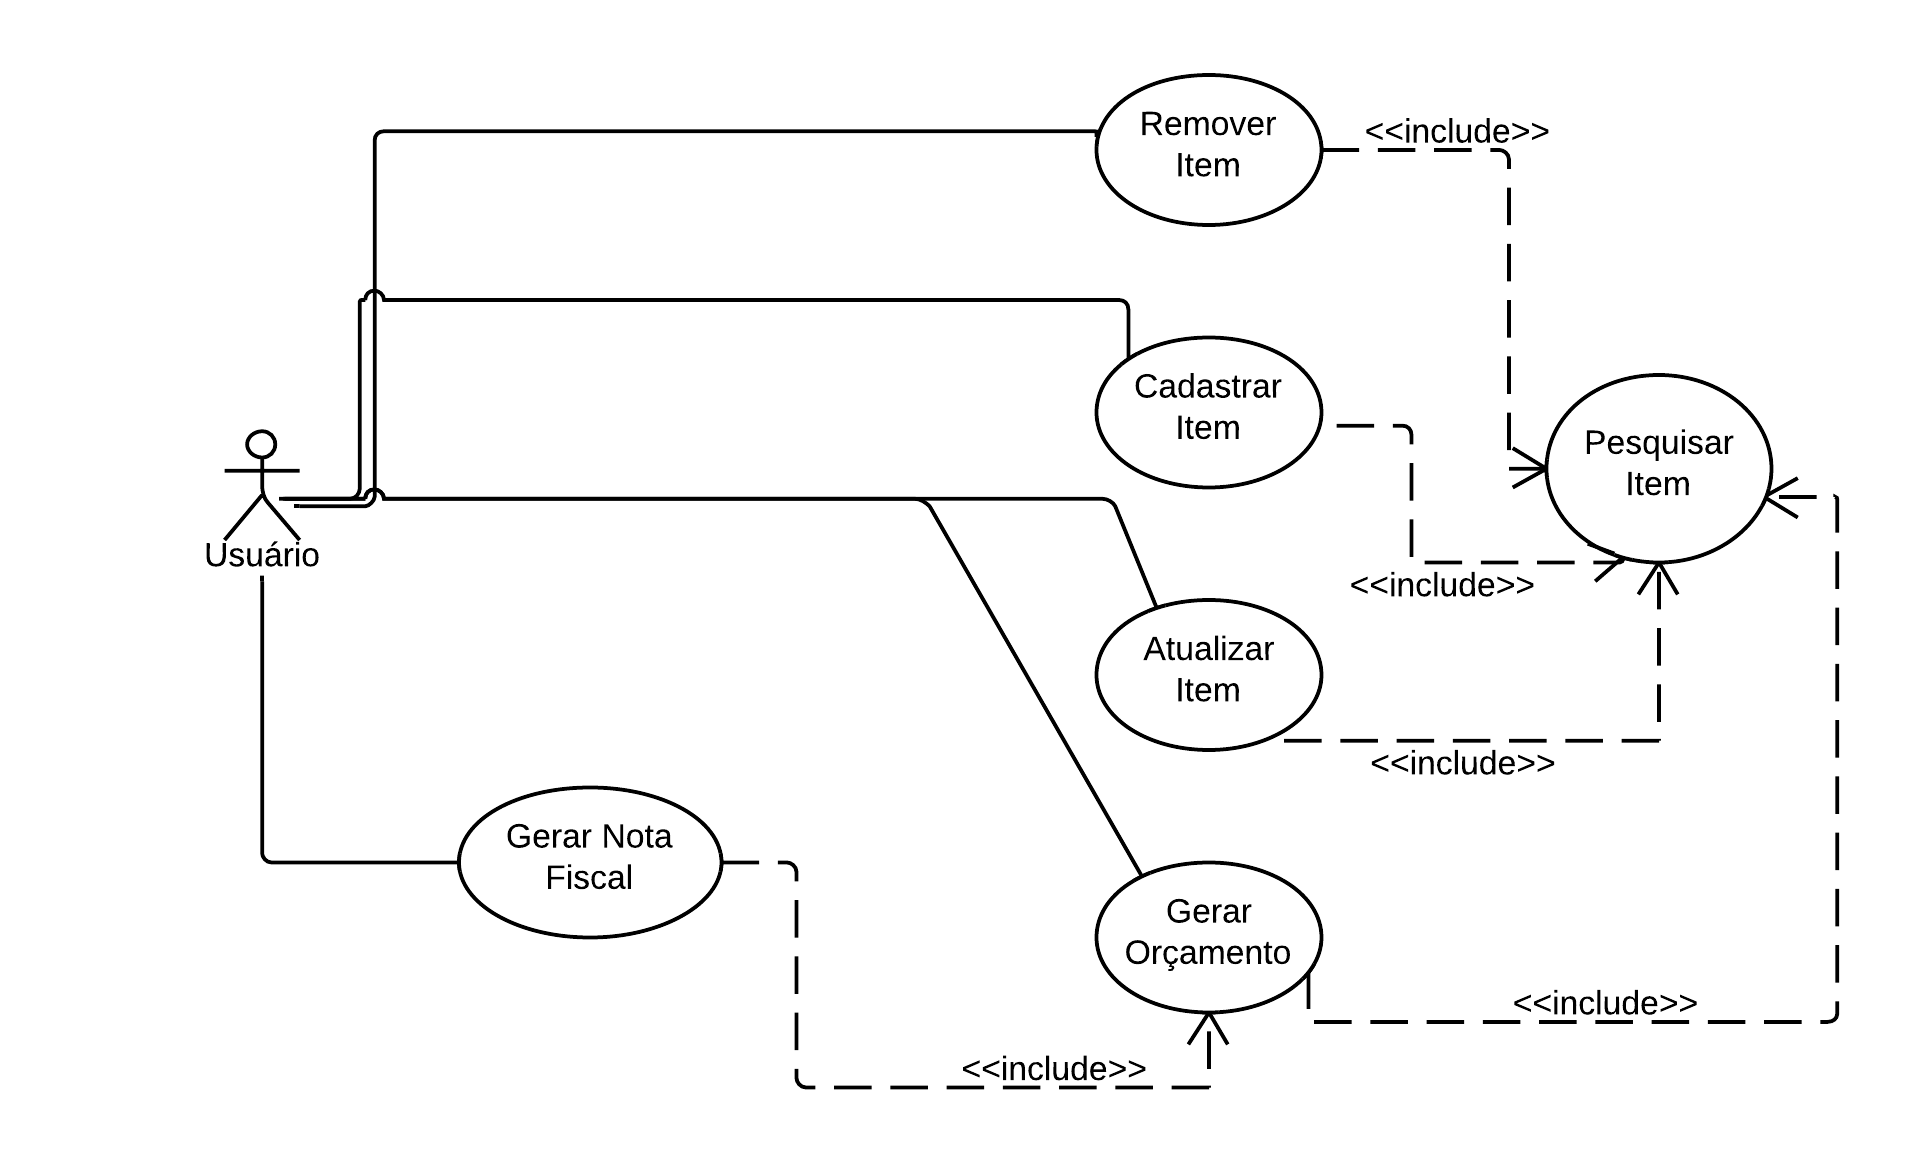
\includegraphics[width=1\textwidth]{pic/casos_de_uso_1.png}
\end{figure}

\begin{figure}[H]
\centering
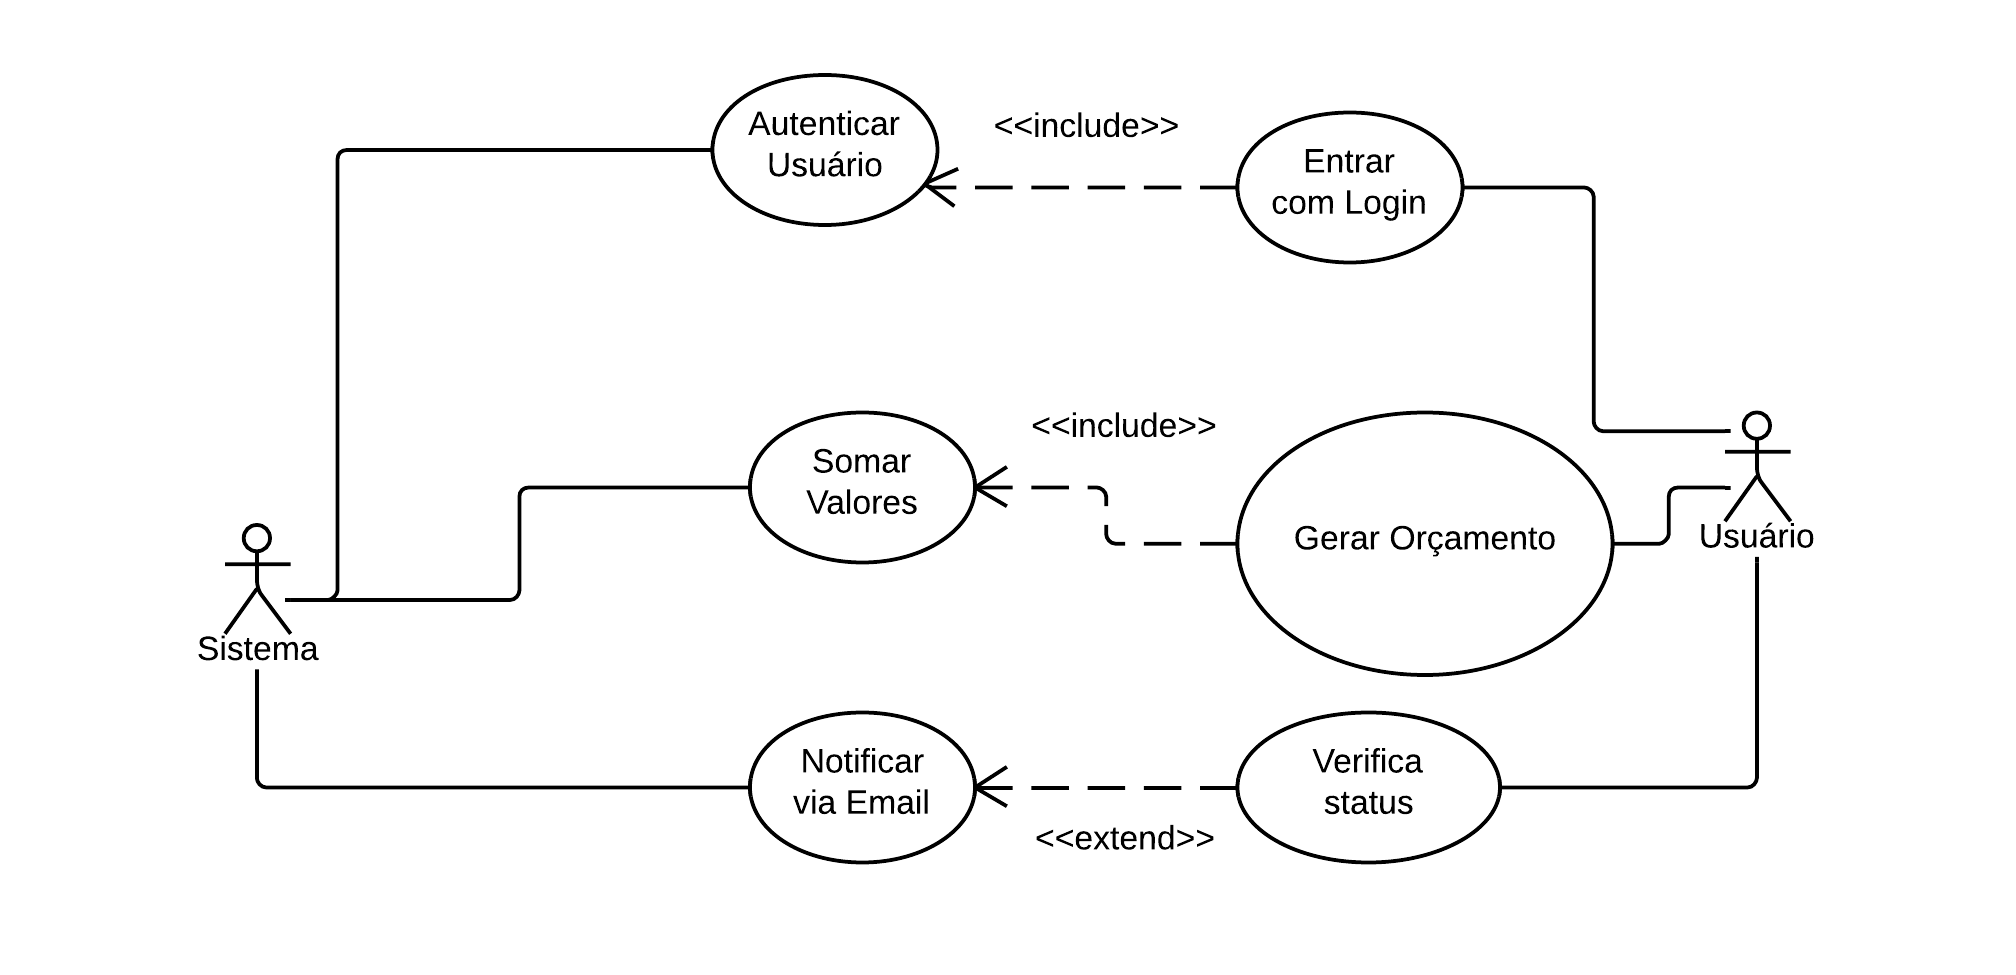
\includegraphics[width=1\textwidth]{pic/casos_de_uso_2.png}
\end{figure}

\subsection{Validação de Requisitos}

Os requisitos definidos pelo cliente foram aprovados pela equipe de desenvolvimento dando então prosseguimento ao desenvolvimento do projeto.

\section{Projeto Arquitetural}

A arquitetura utilizado para a implementação do sistema será a de três camadas por ser a mais utilizado no conceito CRUD. Nota-se que que este tipo de arquitetura proporciona uma maior possibilidade de mudanças em camadas superiores sem afetar de fato as camadas mais abaixo. Para um sistema de cadastro, o fluxo de dados não é grande o que não compromete o desempenho do sistema.

A primeira camada do sistema é a de Apresentação, que é onde toda a parte visual de interação do usuário com o sistema. É a partir dela que o funcionário ou o administrador do sistema tem acesso às funções definidas pelo cliente em alto nível.

A segunda camada, a de controle, é a responsável por toda encapsulação de informação como também o fornecimento de operações feitas pelo sistema tais como validação de usuário, geração de relatórios e orçamentos, calculo de valores entre outros. Nesta camada teremos a transição dos dados fornecidos pelo usuário para a camada de dados, descrita a seguir.

Assim, temos a terceira camada, a de Dados que é a responsável por todo o mapeamento do modelo de dados para a aplicação. Com isso temos funções de farão todo o gerenciamento do banco de dados como também a recuperação dos dados. Abaixo é mostrado como a seguinte arquitetura de comporta:

\begin{figure}[H]
\centering
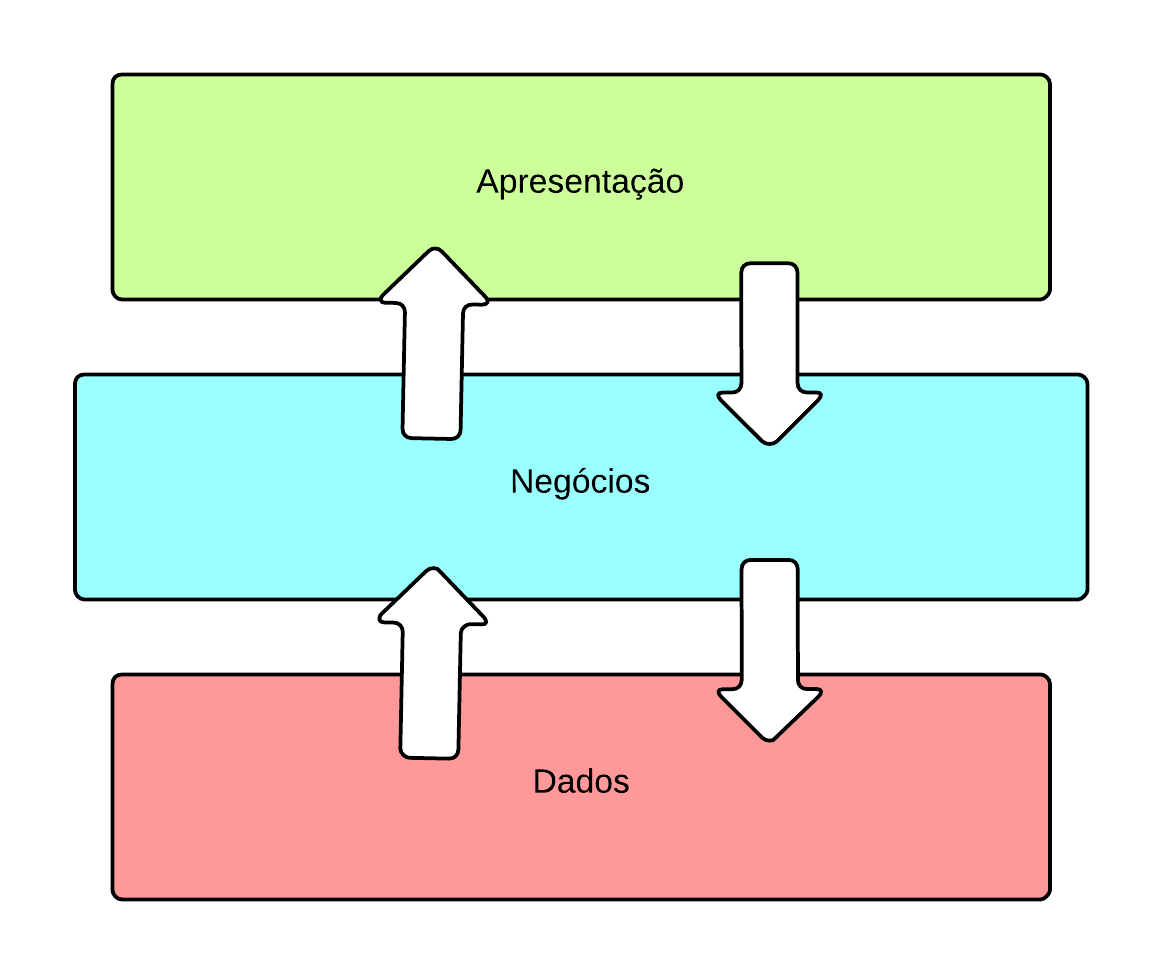
\includegraphics[width=0.7\textwidth]{pic/mvc_1.png}
\end{figure}

Abaixo o segue o diagrama de componentes que constituem o modelo arquitetural de 3 camadas:

\begin{figure}[H]
\centering
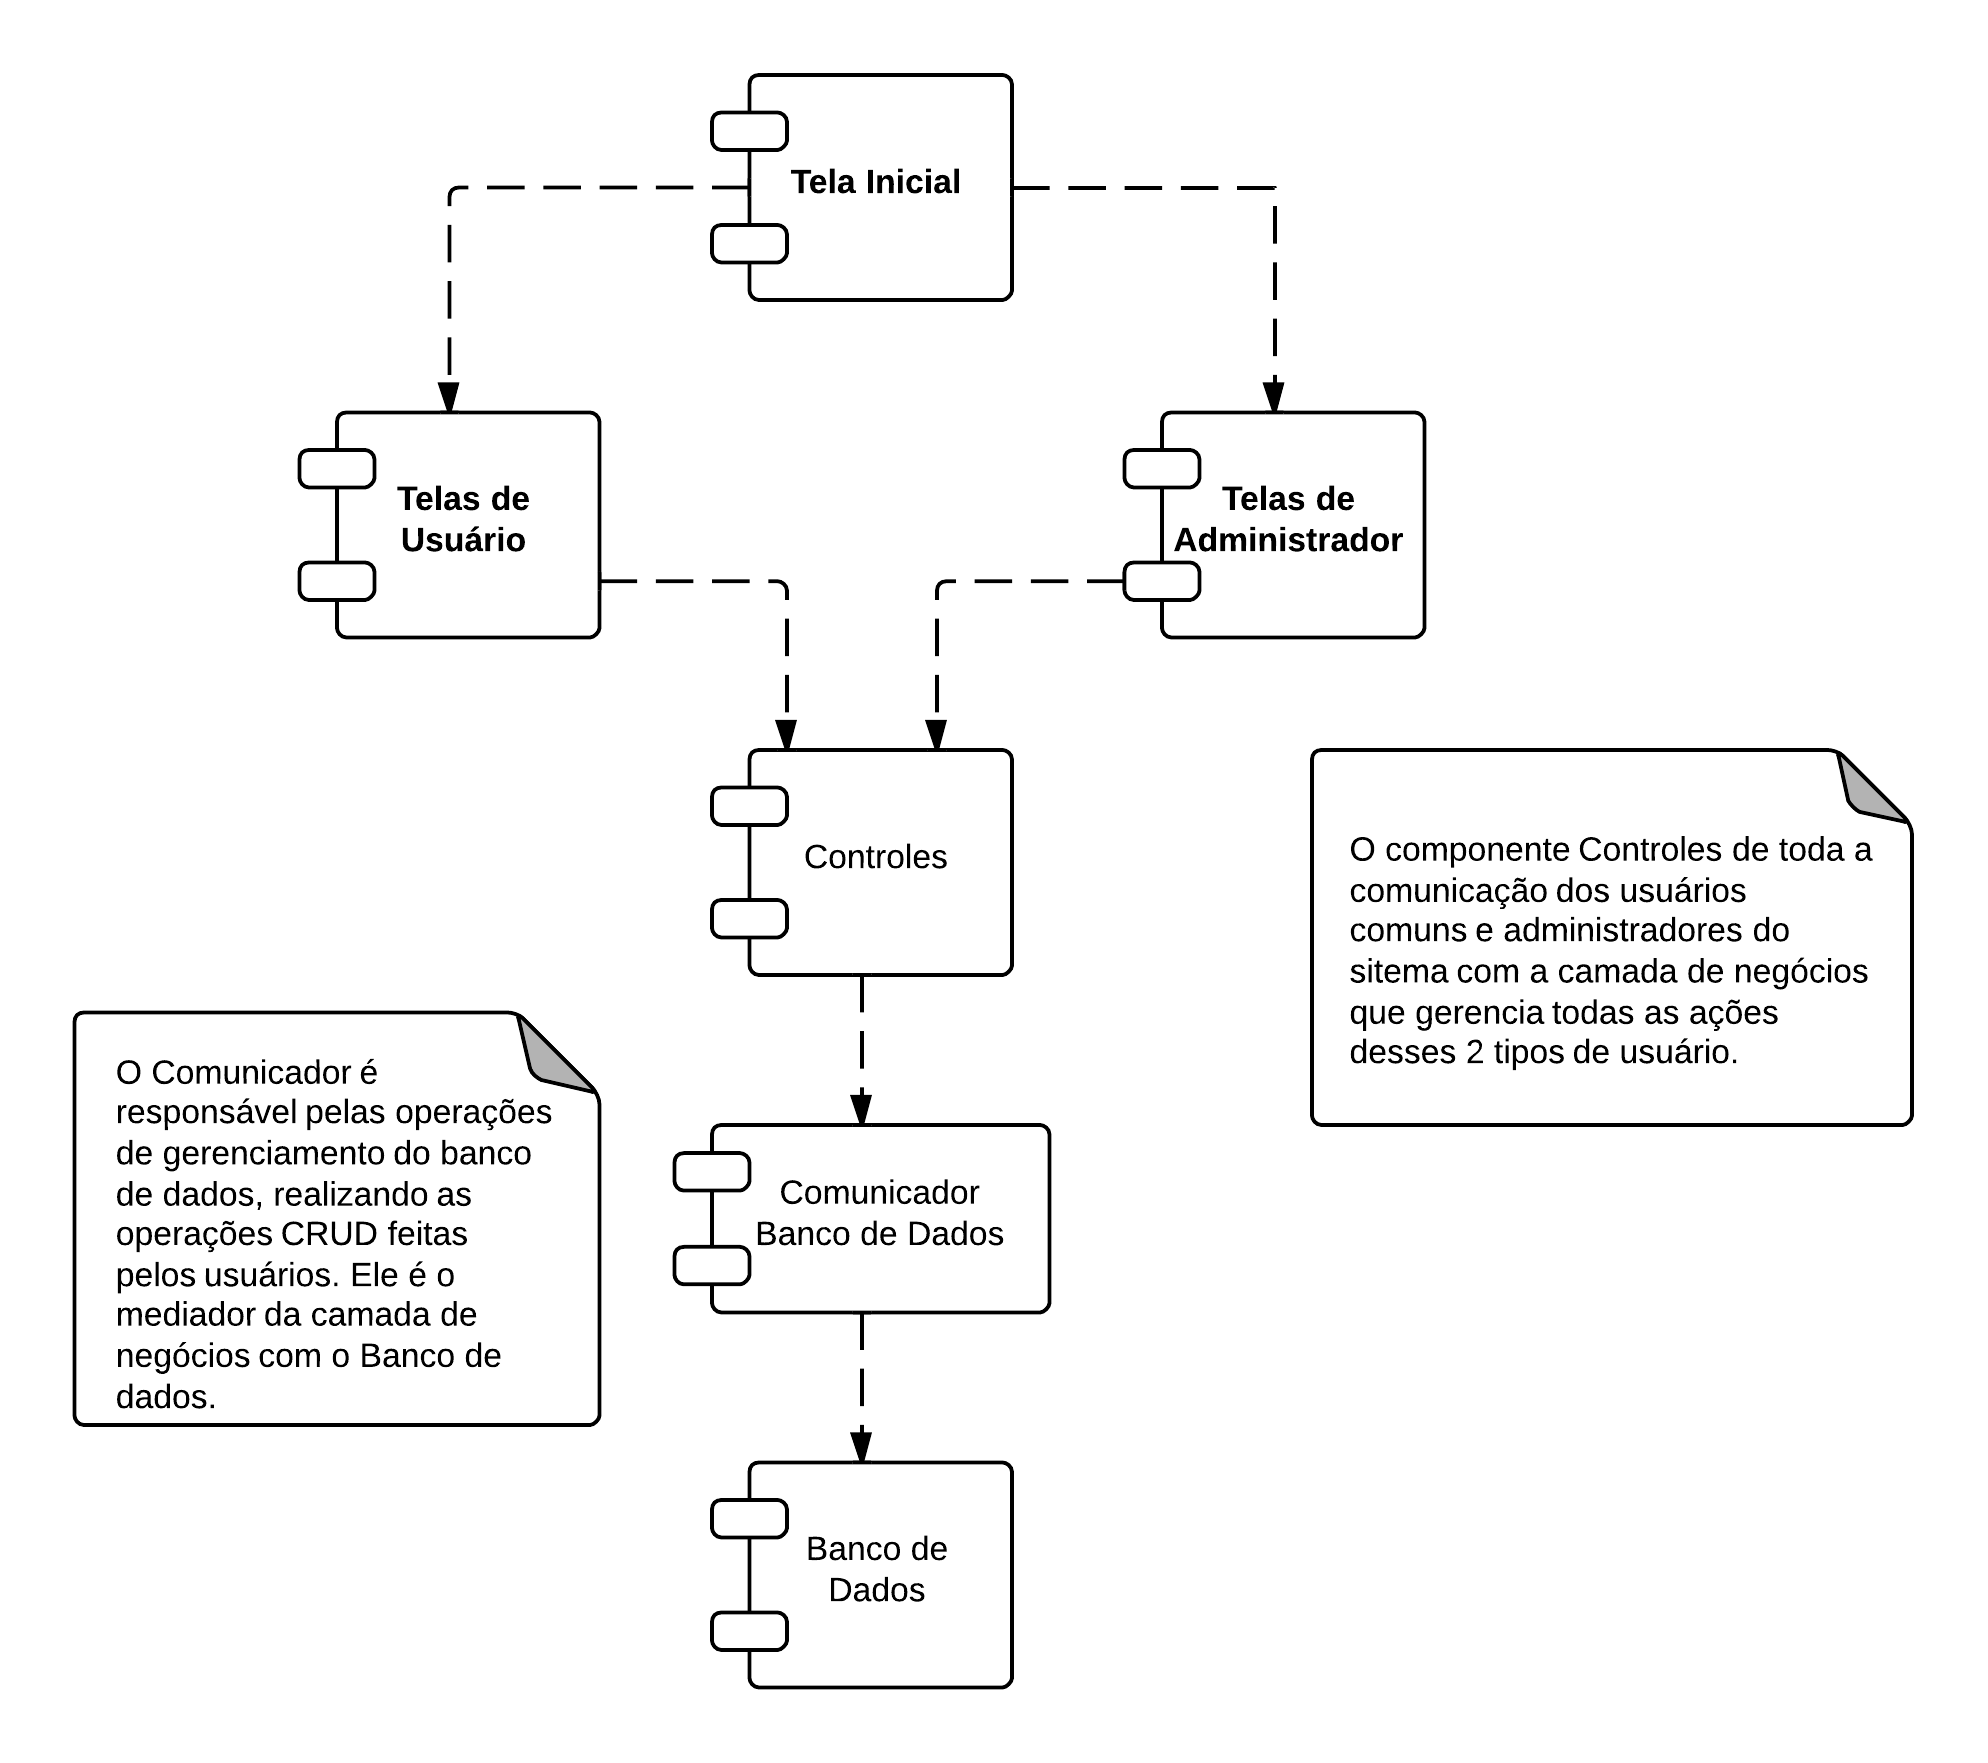
\includegraphics[width=1\textwidth]{pic/componentes.png}
\end{figure}

\section{Detalhes do Projeto}

\subsection{Tecnologias utilizadas}

\textbf{Ambiente}: toda a implementação do sistema foi feita com a IDE Netbeans 7.1.1 com o Java JDK 1.7.

\textbf{Banco de dados}: Para o armazenamento de dados foi utilizado o sistema de bancos de dados MySQL versão 14.14 que provê uma facilidade na comunicação entre os pacotes Java e por ser um software gratuito.

\textbf{Interface Gráfica}: para a construção das telas do sistema, foi utilizado o pacote Swing por ser um pacote nativo da linguagem e pela vantagem do drag and drop para a contsrução da interface.

\textbf{Persistência}: para a persistência de dados foi utilizado o framework Hibernate. Ele possibilita toda a comunicação dos objetos da camada de controle com o banco de dados. Para a configuração do banco, é utilizado um arquivo XML que define as flags e variáveis de inicialização com o MySQL. <ver aqui se precisa de classe repositório>

\textbf{Testes}: para a realização de testes, foi usado a biblioteca jUnit que constitui de funções que possibilitam usar todas as funções implementadas na camada de controle e dados sem necessária dependência de uma interface pronta. Uma vez que temos toda a camada de controle e de dados funcionais fica mais fácil a implementação de uma camada de Visualização que cubra todas os requisitos exigidos pelo cliente

\subsection{Diagrama de Classes}

Abaixo seguem dois diagramas de classes. O primeiro é uma versão simplificada de relacionamento entre os objetos e a segunda uma versão mais detalhada com classes utilizadas pelo Hibernate na camada de dados. Nota-se que na primeira versão algumas classes foram representadas como uma só (camada de Dados e Visualização).

\begin{figure}[H]
\centering
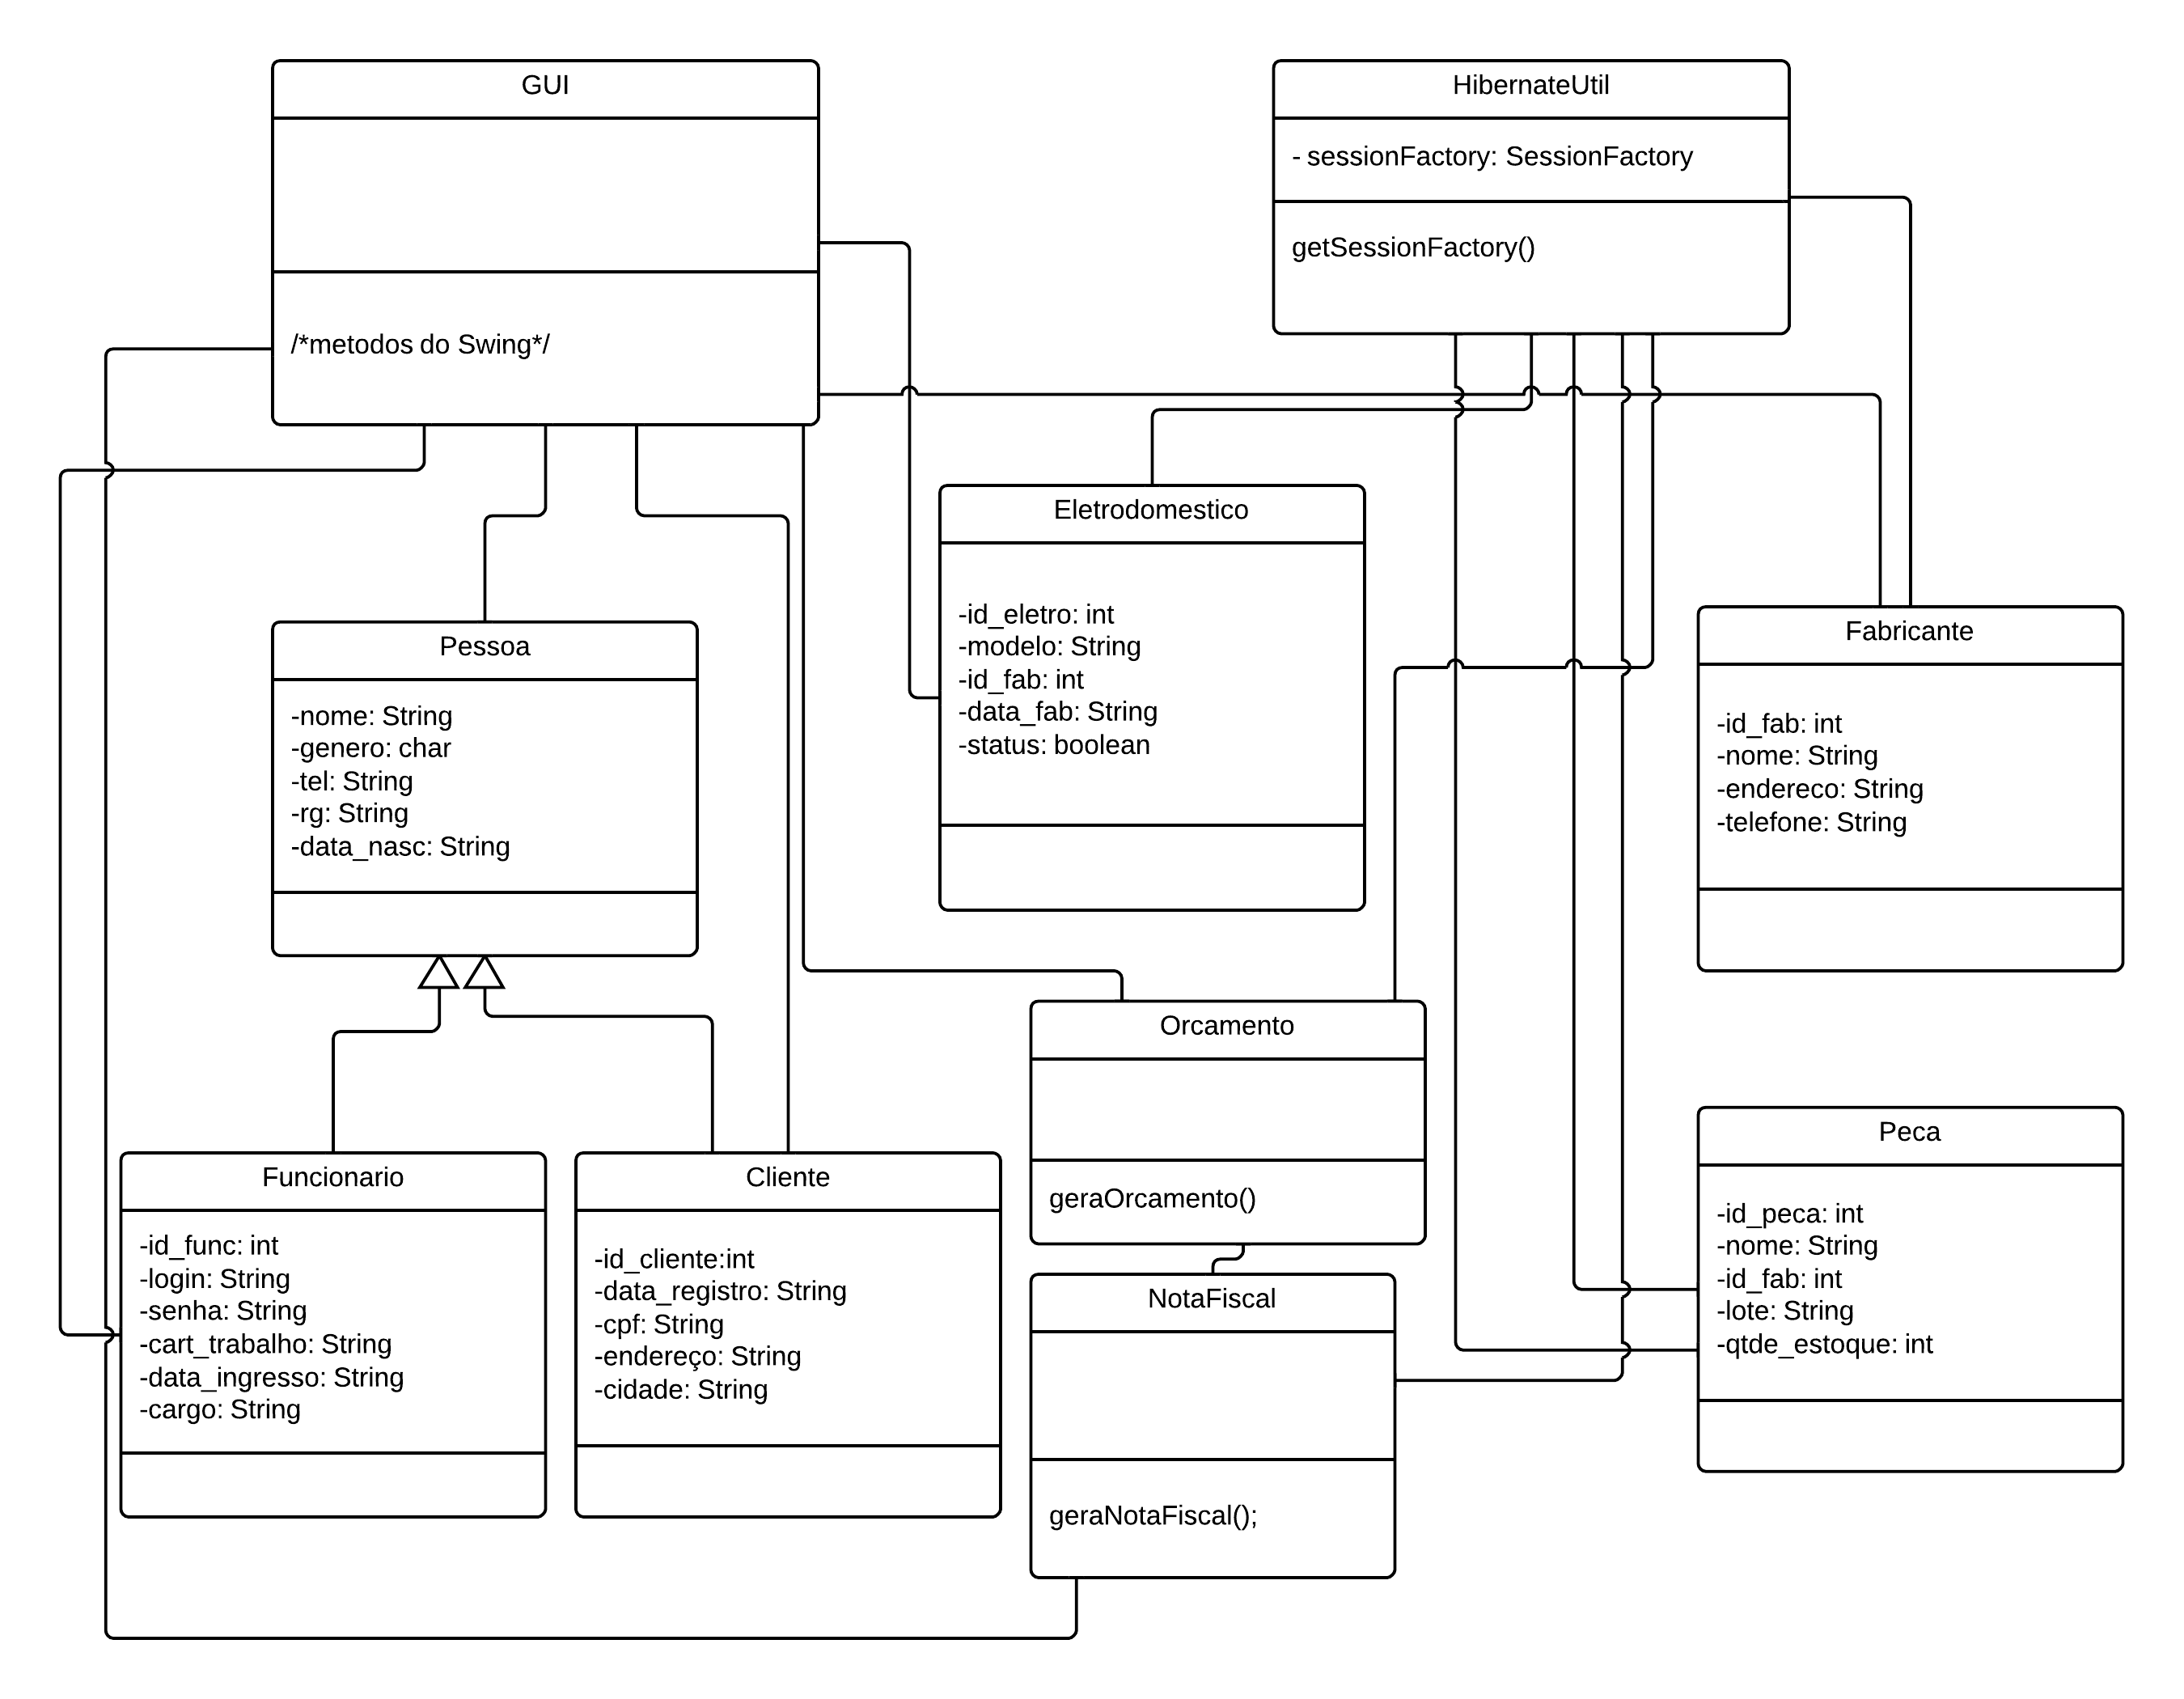
\includegraphics[width=1\textwidth]{pic/classe_11.png}
\end{figure}

\begin{figure}[H]
\centering
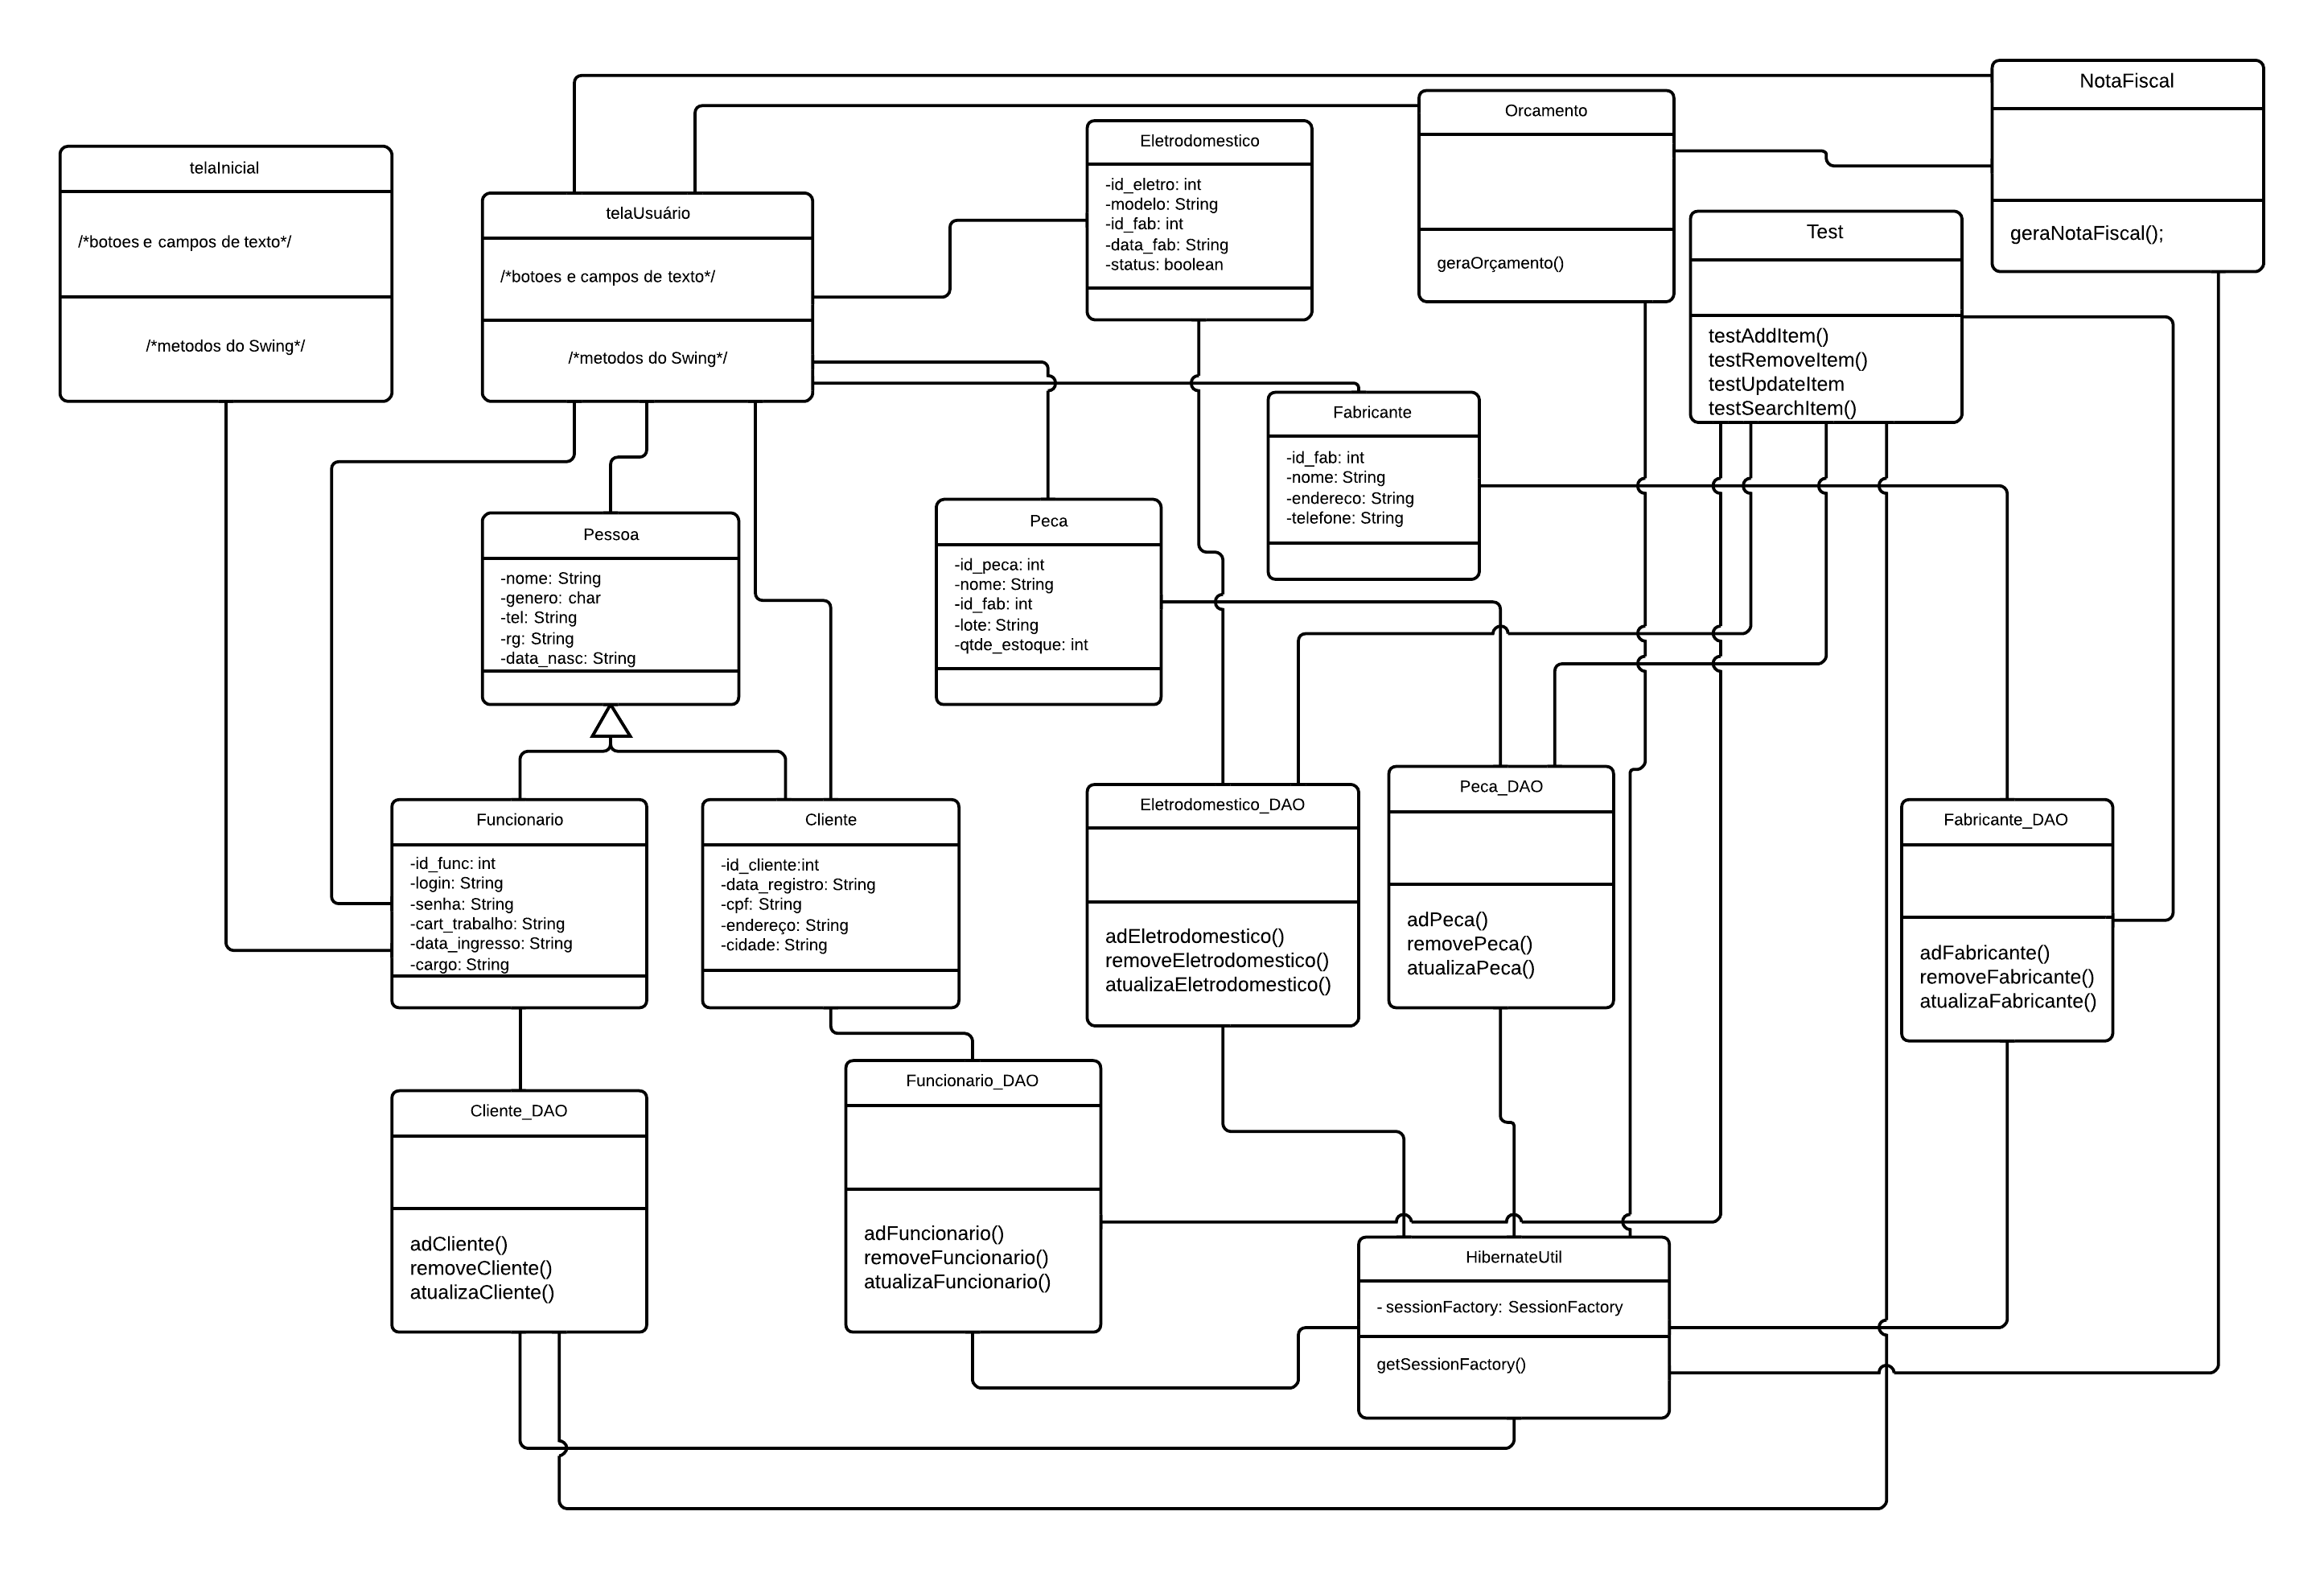
\includegraphics[width=1\textwidth]{pic/classe_2.png}
\end{figure}


\subsection{Diagrama de Sequência}


Abaixo seguem os principais diagramas de sequência para as principais operações de cadastro, remoção e atualização. Para abstrair de forma mais genéricas as classes envolvidas, o uso do nome Subject foi usada já que as mesmas operações são feitas para todas as classes.

\begin{figure}[H]
\centering
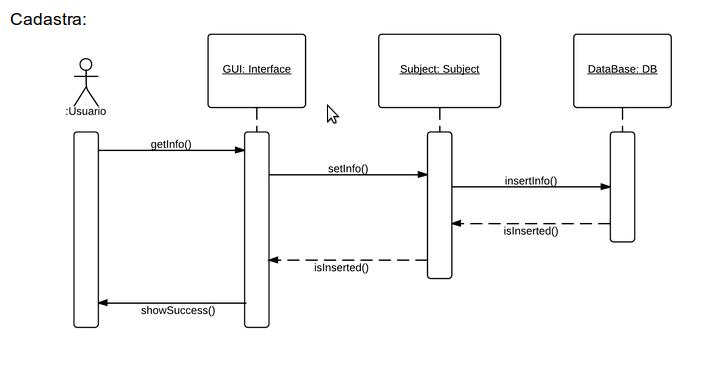
\includegraphics[width=1\textwidth]{pic/sequencia_1.jpeg}
\end{figure}

\begin{figure}[H]
\centering
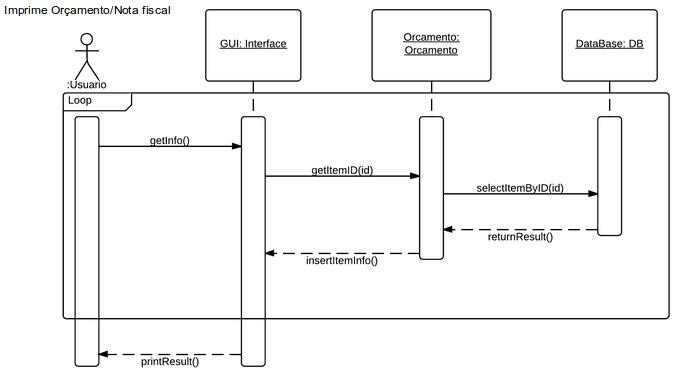
\includegraphics[width=1\textwidth]{pic/sequencia_2.jpeg}
\end{figure}

\subsection{Diagrama de pacotes}

Abaixo segue os pacotes utilizados na implementação, tais como aqueles criados para encapsular as classes utilizadas e das bibliotecas que farão a comunicação com o banco de dados e a criação da interface.

\begin{figure}[H]
\centering
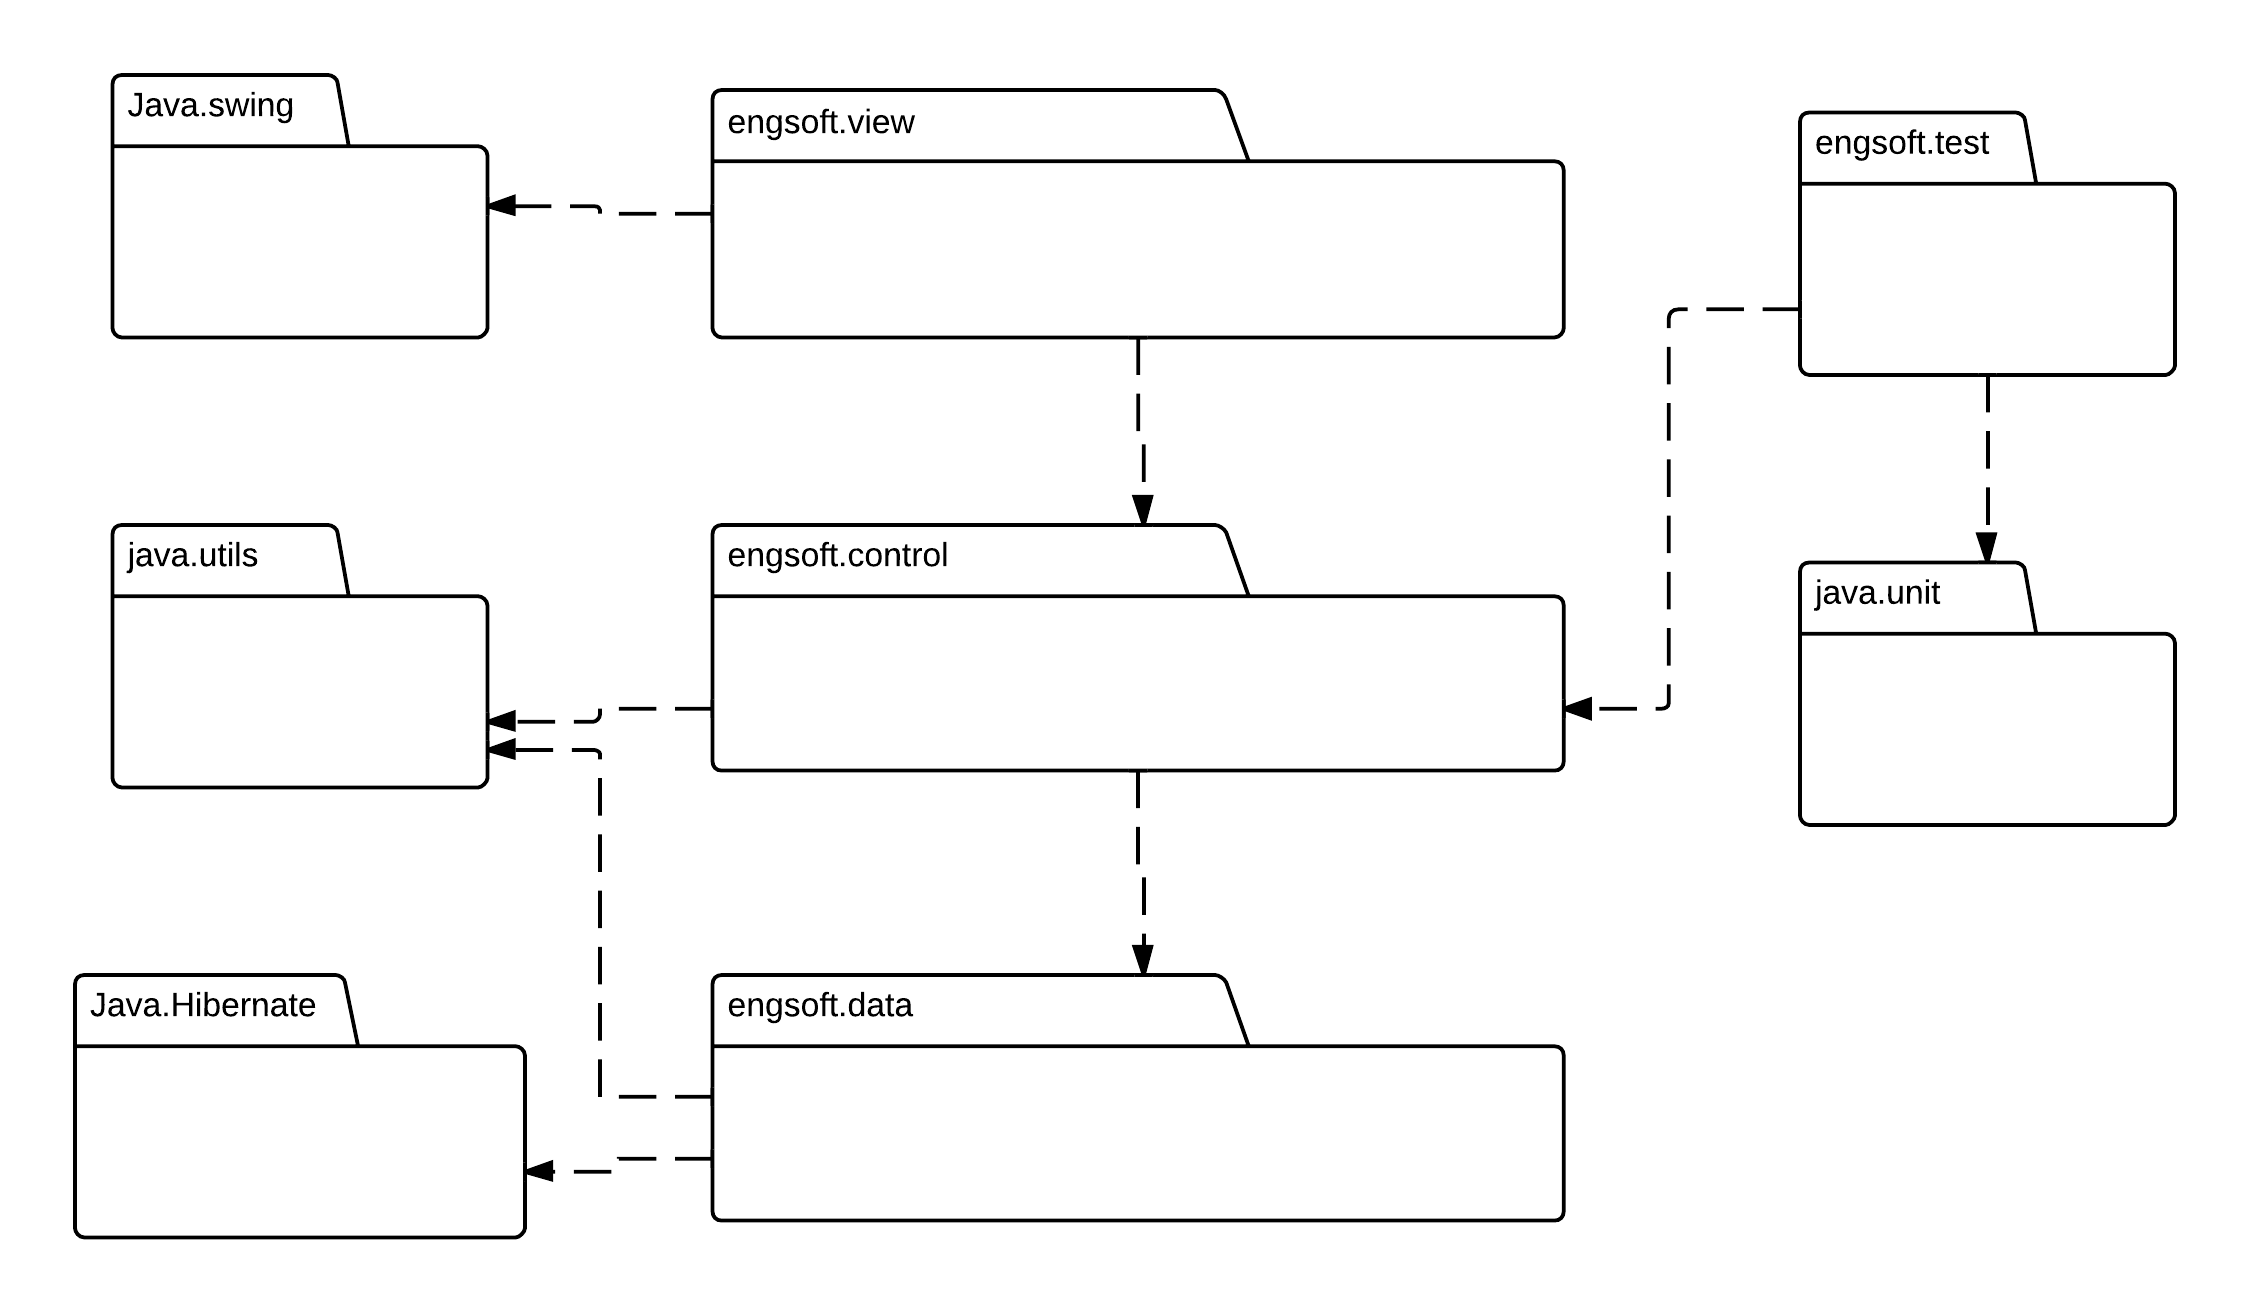
\includegraphics[width=1\textwidth]{pic/pacotes.png}
\end{figure}

\subsection{Diagrama de atividades}

Abaixo os diagramas de atividades para as principais atividades realizadas. Nota-se que foram destacadas apenas as atividades mais críticas.

\begin{figure}[H]
\centering
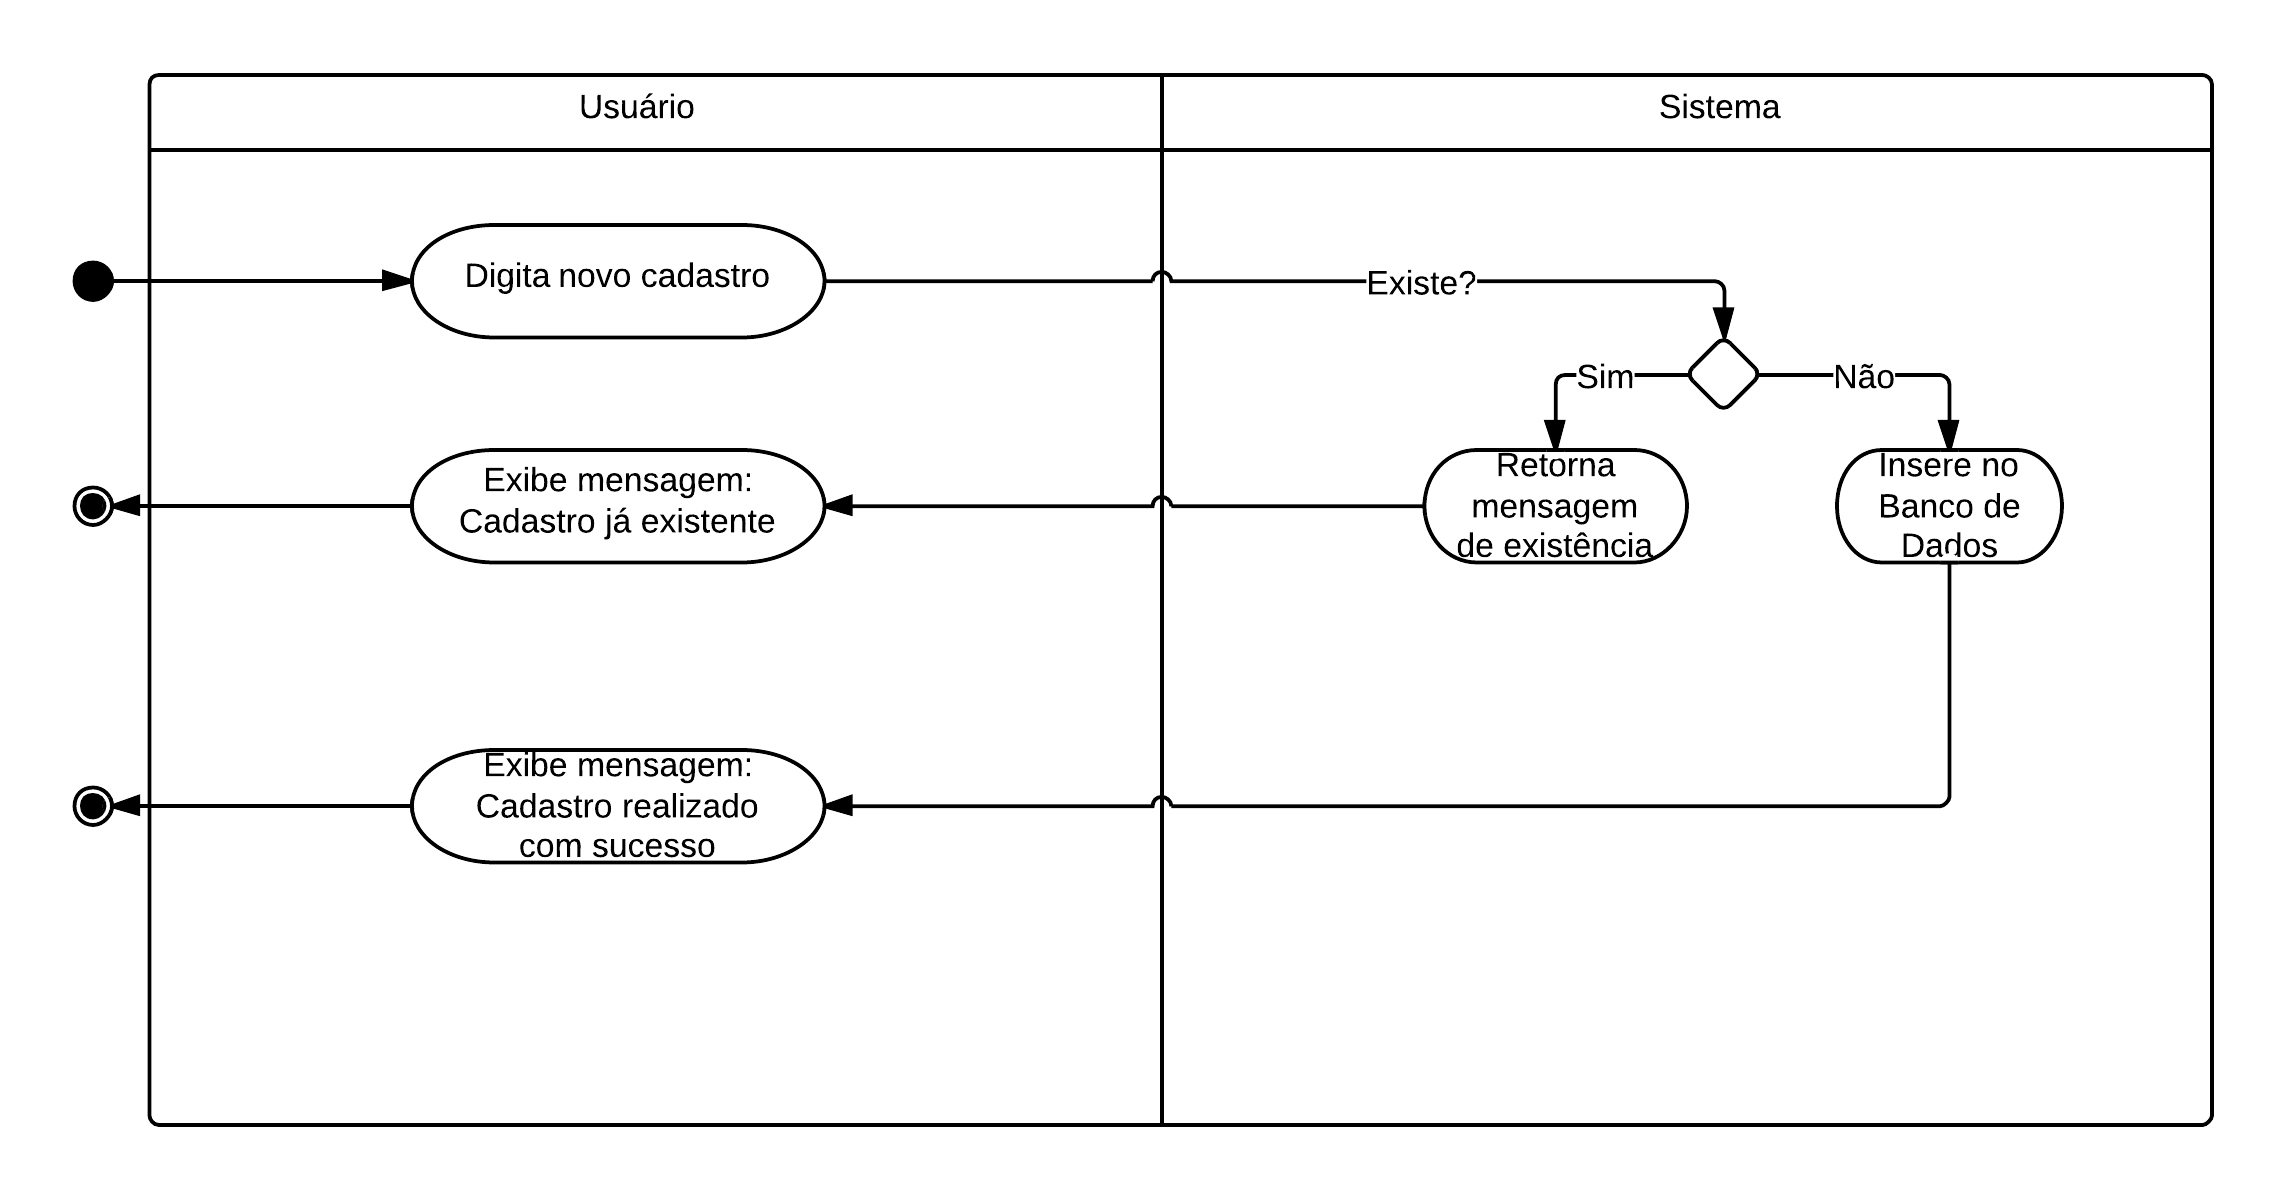
\includegraphics[width=1\textwidth]{pic/atividades_1.png}
\end{figure}

\begin{figure}[H]
\centering
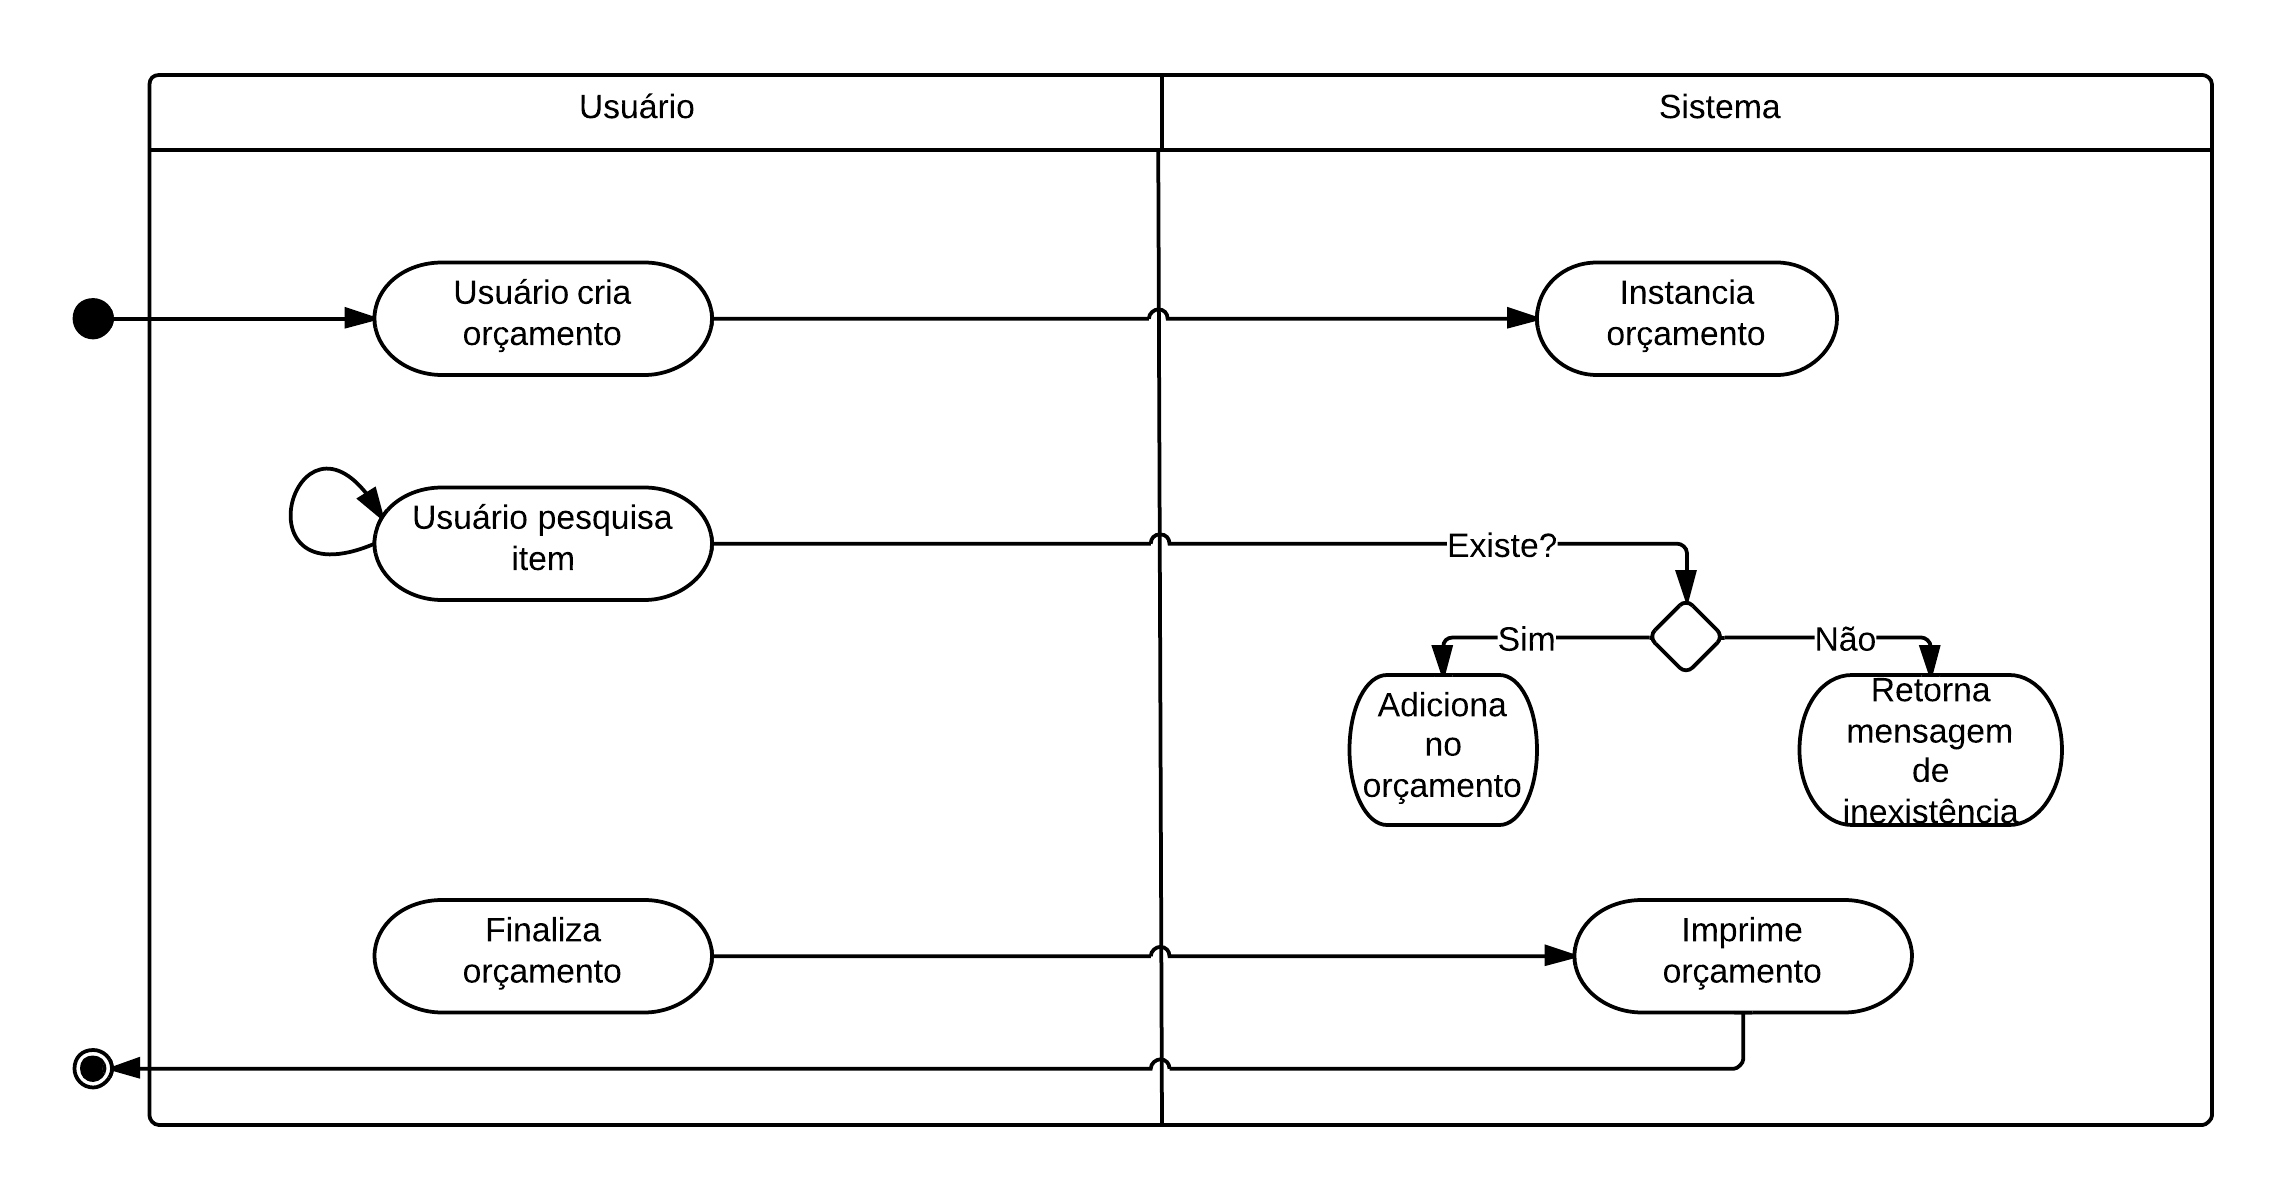
\includegraphics[width=1\textwidth]{pic/atividades_2.png}
\end{figure}

\section{Implementação:}


Toda a implementação da parte lógica foi concluída para as funções CRUD como as de cadastro, remoção e atualização de cliente, peça, funcionário e fabricante. Funções da interface gráfica não foram totalmente completadas, porém foram detalhadas nessa documentação para fins didáticos. A conclusão de uma interface gráfica demanda de várias horas assim como a constante avaliação do cliente o que pode levar tempo para a total implementação. Para cobrir os testes foi usado a biblioteca jUnit. Desse modo podemos cobrir todos os testes necessários sem a presença de uma interface completamente pronta. Isso nos dá uma abstração dos possíveis casos de uso do sistema.

\section{Conclusão}

O trabalho desenvolvido para a disciplina de Engenharia de Software constituiu na implementação de um sistema para uma oficina de eletrodomésticos. Nele foram abordados todos os processos que normalmente são realizados pelas empresas para a implementação de um software e que foram aprendidos no decorrer da matéria. 

A elaboração de um documento completo, com a construção de diagramas UML foi de suma importância, já que na maior parte das matérias do curso de Ciência da Computação temos noções apenas da parte da programação não nos dando um detalhamento das etapas de um sistema mais complexo como a disciplina de Engenharia de Software nos dá. 

Parte principal de um software é a sua especificação junto com a análise de requisitos, pois nela que se consegue determinar o quanto será necessário se esforçar para conseguir terminar o projeto e obter um software funcionando com qualidade, aspecto hoje que é totalmente negligenciado pelas empresas. Demandas inconsequentes, clientes que não sabem o que querem junto com desenvolvedores que não trabalham a parte de especificação de um software somam um conjunto precário que resultará em um sistema ruim. 

Estimar quanto se gasta e quanto vai custar um software também é um dos pontos mais complicados hoje em dia, a falta de organização das empresas e de planejamento, faz com que mensurar quanto é gasto e quanto será necessário para executar um projeto seja uma tarefa complicada. 

Engenharia de software mostrou o quanto é importante o planejamento, tanto para desenvolvedores quanto para clientes, onde um bom planejamento vai gerar um bom projeto, com deadlines viáveis e um sistema bem estruturado livre de falhas e garantirá ao cliente um sistema que atenda a sua demanda, solucione o seu problema e o principal um software de qualidade.

Portanto o trabalho cumpriu satisfatoriamente seus objetivos no desenvolvimento do sistema proposto e proporcionou bastante experiência aos envolvidos.

\section{Referências}

\begin{enumerate}
\item Sommervile, Iam. Engenharia de Software. Pearson - 9ª ed. 2011
\item Pressman, Roger. Engenharia de Software: Uma Abordagem Profissional. Bookman, 7ª ed.
\item Booch, G., Rumbaugh, J., Jacobson, I. UML, Guia do Usuáario. 2ª ed., Editora Campus, 2005
\end{enumerate}


\end{document}
